\documentclass{Phyport}

\usepackage{hyperref}
\hypersetup{
    colorlinks=true,
}
\usepackage{amsmath, amsthm, amssymb, amsfonts}
\usepackage{esint}
\usepackage{nicematrix}
\usepackage{extarrows}
\usepackage{graphicx}
\usepackage{enumitem}
\usepackage{multirow, booktabs}
\usepackage{caption}
\usepackage{float}
\usepackage[dvipsnames]{xcolor}
\usepackage[english]{babel}
\usepackage{bm}
\usepackage{cite}

\exname{金属材料杨氏模量的测定} %实验名称
\extable{14} %实验桌号
\instructor{张贯乔} %指导教师
\class{github} %班级
\name{MJ} %姓名
\stuid{2025} %学号

\nyear{2025} %年
\nmonth{10} %月
\nday{27} %日
\nweekday{一} %星期几

\redate{} %如有实验补做，补做日期
\resitu{} %情况说明：

\begin{document}
\setcounter{page}{0}
\makecover

\section{预习报告（10分）}

\subsection{实验综述（5分）}

杨氏模量是描述固体材料抵抗弹性形变能力的重要物理参数，反映了材料的刚度。本实验测量金属的杨氏模量：
\[
E = \frac{F \cdot L}{S \cdot \Delta L}
\]
在数值上等于金属产生单位应变时的应力，并且与金属丝的材料有关，与外力及物体的形状无关。

实验中采用灵敏度较高的光杠杆法以及小量近似原理来测量金属丝在拉伸载荷下产生的微小伸长量，从而精确计算出该金属材料的杨氏模量。
光杠杆将金属丝伸长导致的微小垂直位移转化为光杠杆镜的微小转角，标尺经光杠杆镜反射后在望远镜中成像。
\begin{figure}[htbp!]
    \centering
    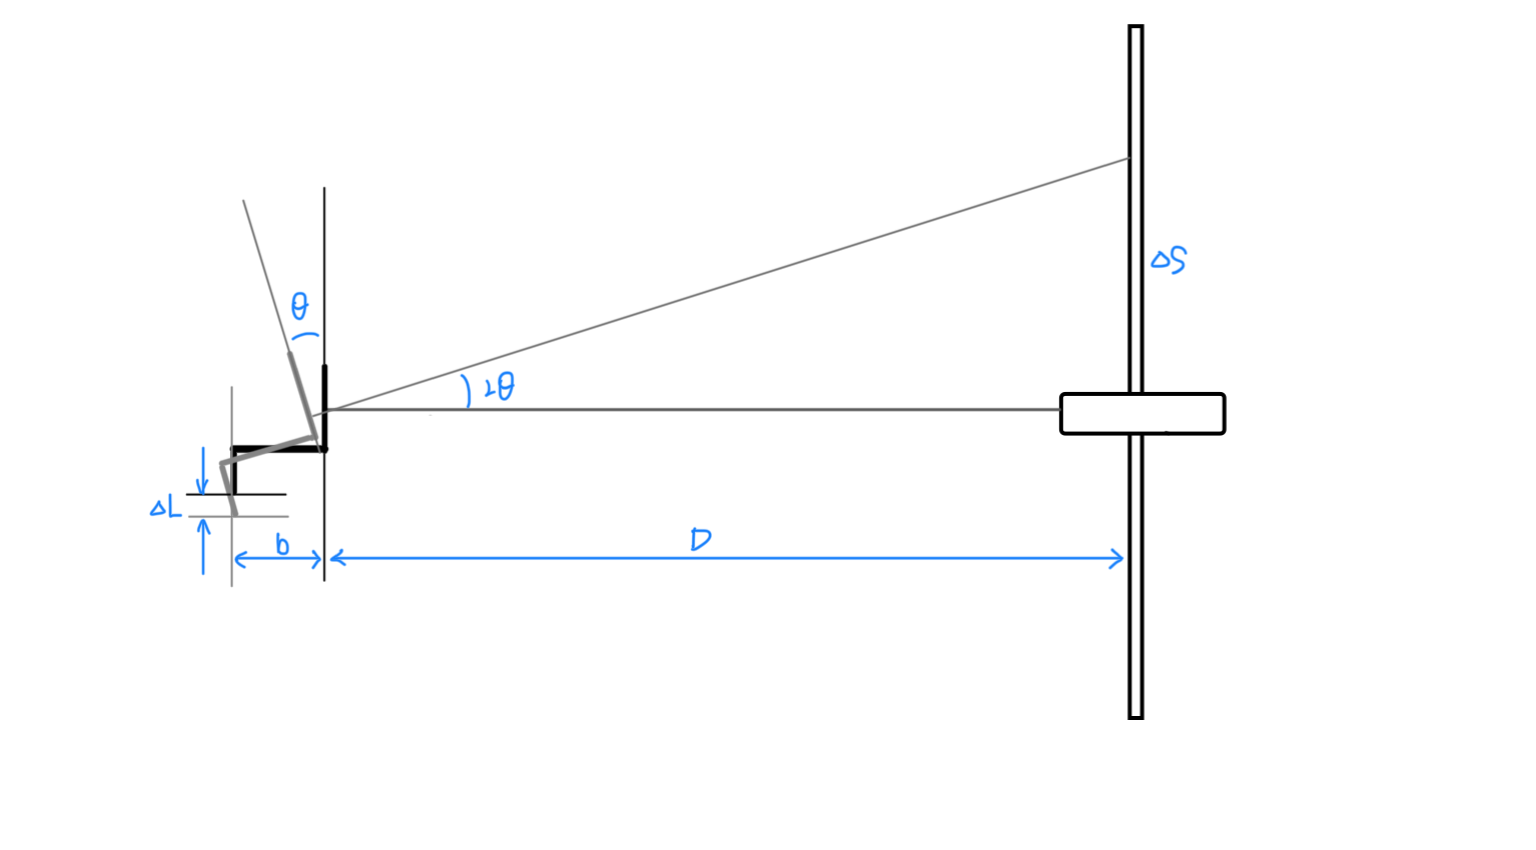
\includegraphics[width=0.6\textwidth]{model_display.png}
\end{figure}

根据光学原理和光路图，标尺上的读数位移与金属丝伸长量之间存在放大关系：
\[
\Delta S = \frac{2D}{b} \cdot{\Delta L}
\]

对于其他量进行多次测量取平均值，实验的测量公式为：
\[
E = \frac{8 DFL}{\pi d^2 b \cdot{\Delta s}}
\]

测量时，先施加一个初始载荷以拉直金属丝并消除系统误差，随后逐级增加砝码，待载荷稳定后读数。完成加载过程后，
应以相同的步长逐级卸载砝码，并记录卸载时的读数。通过加载和卸载的两组数据，求得对应于质量增量的标尺读数变化量的平均值，
以消除系统误差和轻微的滞后效应。

在实验过程中，观察到每当砝码改变时，望远镜中标尺的读数发生清晰可辨的移动。并且在弹性限度内，每增加相同的质量，
读数移动的距离近似相等；在卸载砝码的过程中，标尺读数会沿着与加载时基本相同的路径逆向移动，并在最终回到初始载荷时的读数附近。


\subsection{实验重点（3分）}

本实验重点主要在于理解杨氏模量的具体定义以及测量原理；掌握光学放大原理和用光杠杆法测量微小长度的原理和方法；掌握数据分析和处理的方法。

\subsection{实验难点（2分）}

本实验难点主要在于微小长度的测量误差必须控制在更小的范围之内，否则放大后会显著影响结果；光杠杆与标尺必须稳定，
防止外界扰动和温度导致热胀冷缩等干扰标尺读数以及确保金属丝的形变完全由拉力引起。

\section{原始数据（20分）}

\begin{figure}[htbp!]
    \centering
    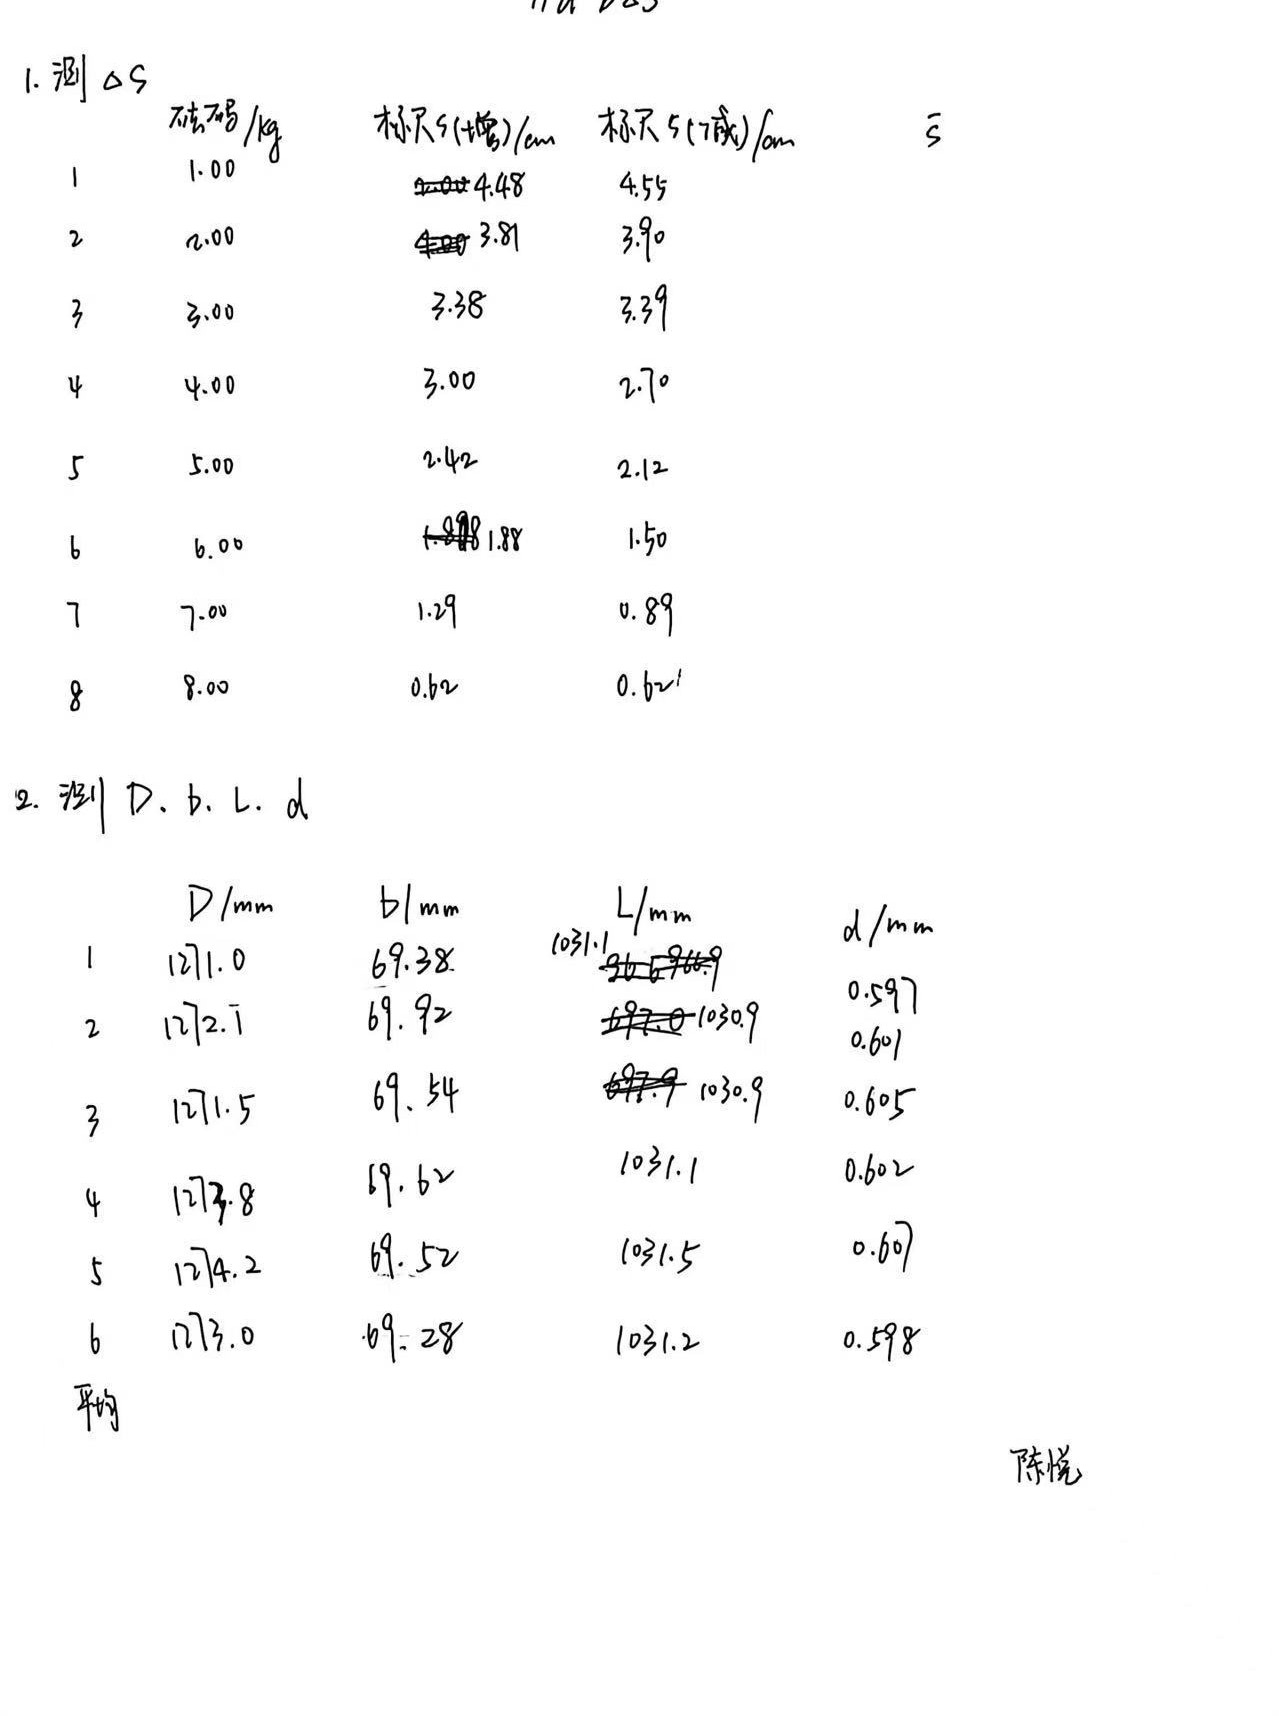
\includegraphics[width=0.7\textwidth]{raw_data.jpg}
\end{figure}

\section{结果与分析（60分）}
\subsection{数据处理与结果（30分）}

1.观测钢丝伸长量

\begin{table}[htbp!]
    \centering
    \begin{tabular}{|l|l|l|l|l|}
        \hline
        实验次数 & 砝码 $/ kg$ & 标尺读数 $s$ （增）$/ cm$ & 标尺读数 $s$ （减） $/ cm$ & 平均值 $/ cm$ \\ 
        \hline
        1 & 1.00 & 4.48 & 4.55 & 4.52 \\ 
        2 & 2.00 & 3.81 & 3.90 & 3.86 \\ 
        3 & 3.00 & 3.38 & 3.39 & 3.38 \\
        4 & 4.00 & 3.00 & 2.70 & 2.85 \\ 
        5 & 5.00 & 2.42 & 2.12 & 2.27 \\
        6 & 6.00 & 1.88 & 1.50 & 1.66 \\
        7 & 7.00 & 1.29 & 0.89 & 1.09 \\
        8 & 8.00 & 0.62 & 0.62 & 0.62 \\
        \hline
    \end{tabular}
\end{table}

采用作图法处理金属丝的伸长量数据，通过MATLAB线性拟合 $mg$ 与 $\Delta s$ ， 得到拟合斜率
\[
\bar{k} = fit(\frac{mg}{\Delta s}) = 1.7539 \times 10^3 N/m
\]
以及拟合斜率的不确定度
\[
\Delta k = 3 \Delta [fit(\frac{mg}{\Delta s})] = 6.7056 \times 10 N/m
\]

\begin{figure}[htbp!]
    \centering
    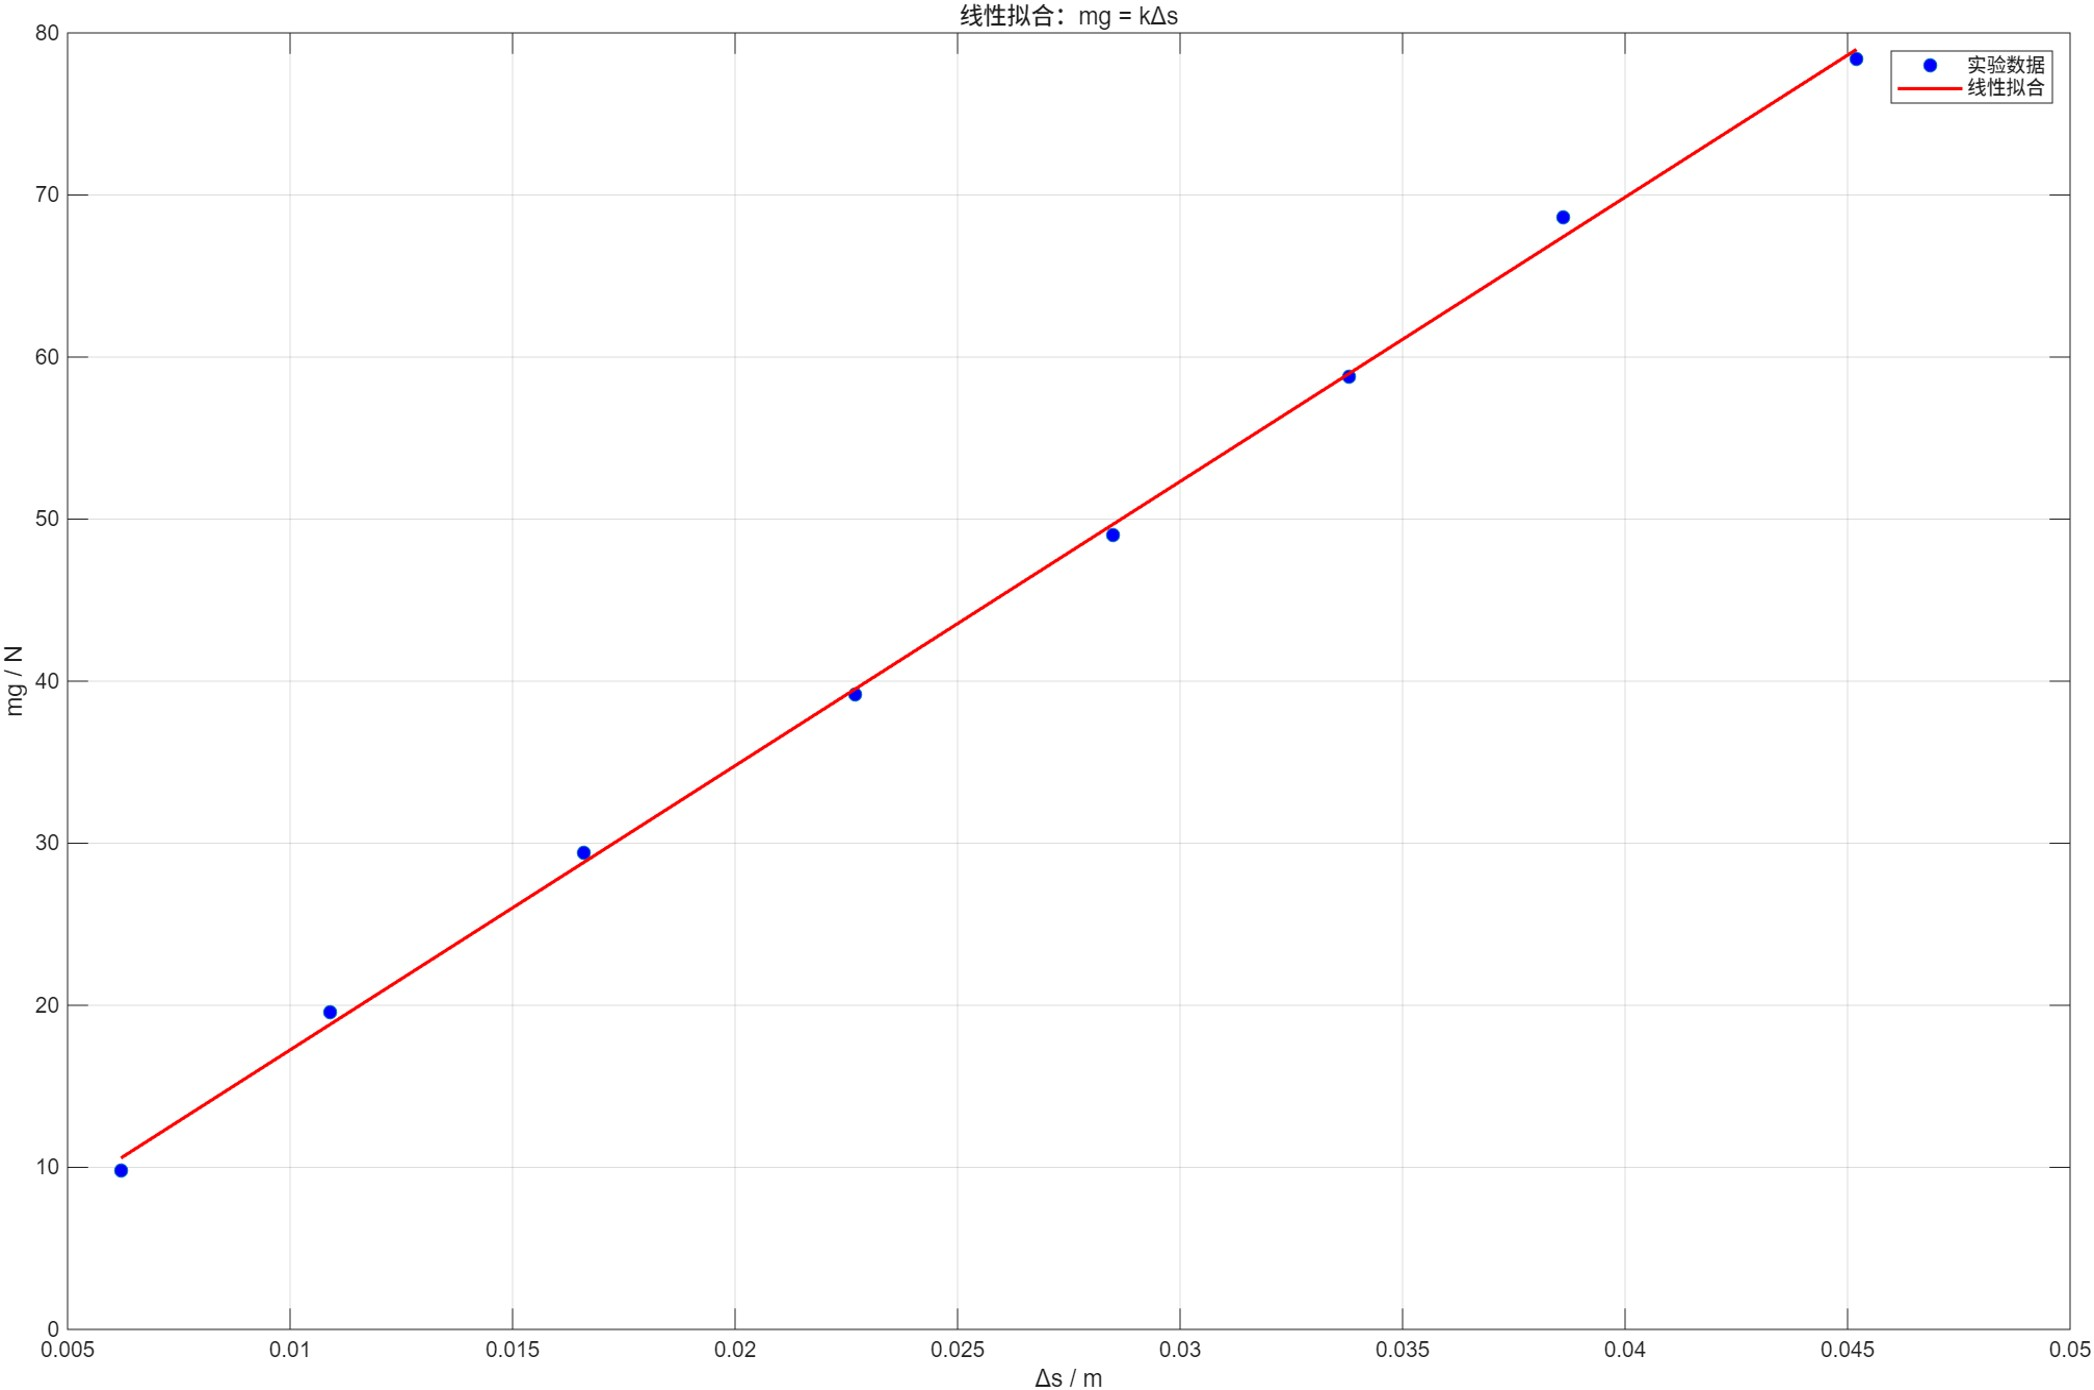
\includegraphics[width=0.8\textwidth]{fit_result.jpeg}
\end{figure}

2.测量各长度

对于 $D$ 、 $B$ 、$l$ 、$d$ 进行六次测量并各自取平均值。
\begin{table}[htbp!]
    \centering
    \begin{tabular}{|l|l|l|l|l|}
        \hline
        物理量 & $D / mm$ & $b / mm$ & $L / mm$ & $d / mm$ \\ 
        \hline
        1 & 1271.0 & 69.38 & 1031.1 & 0.597 \\ 
        2 & 1272.1 & 69.92 & 1030.9 & 0.601 \\ 
        3 & 1271.5 & 69.54 & 1030.9 & 0.605 \\
        4 & 1273.8 & 69.62 & 1031.1 & 0.602 \\ 
        5 & 1274.2 & 69.52 & 1031.5 & 0.607 \\
        6 & 1273.0 & 69.28 & 1031.2 & 0.598 \\
        \hline
        平均值 & 1272.6 & 69.54 & 1031.1 & 0.602 \\
        \hline
    \end{tabular}
\end{table}

因为实验时没有注意记录使用仪器的允差，所以用 $A$ 类不确定度代替总不确定度，根据贝塞尔公式
\[
u(\bar{x}) = \sqrt{\frac{\sum_{i=1}^n (x_i - \bar{x})^2}{n(n-1)}}
\] 
分别计算各长度的不确定度
\begin{table}[htbp!]
    \centering
    \begin{tabular}{|l|l|l|l|l|}
        \hline
        物理量 & $D / mm$ & $b / mm$ & $L / mm$ & $d / mm$ \\ 
        \hline
        不确定度 & 0.5 & 0.09 & 0.09 & 0.002 \\ 
        \hline
    \end{tabular}
\end{table}

3.计算金属丝的杨氏模量

把拟合得到的斜率和各长度测量的平均值代入公式，得到：
\[
\bar{E} = \frac{8 \bar{D} \bar{L}}{\pi \bar{d}^2 \bar{b}} \cdot \bar{k} = 2.32 \times 10^{11} Pa
\]
分析杨氏模量的不确定度，根据传导关系有
\[
\frac{\Delta E}{\bar{E}} = \sqrt{(\frac{\Delta k}{\bar{k}})^2 + (\frac{\Delta L}{\bar{L}})^2 + (\frac{\Delta D}{\bar{D}})^2
+ (\frac{2 \Delta d}{\bar{d}})^2 + (\frac{\Delta b}{\bar{b}})^2}
\]
求出 $\Delta E = 0.09 \times 10^{11} Pa$

金属丝的杨氏模量为
\[
E = \bar{E} \pm \Delta E = (2.32 \pm 0.09) \times 10^{11} Pa 
\]

\subsection{误差分析（20分）}

根据不确定度分析和最终测量的金属丝杨氏模量结果，实验基本达到了目的，主要误差来源可能有：
\begin{itemize}
    \item 标尺读数分散性相对大，没有更好地满足线性关系，可能是因为测量过程中光杠杆受环境干扰不完全稳定以及改变载荷后金属丝的形变没有完全稳定；
    \item 测量较小的长度时读数误差比较大，特别是用螺旋测微器测量金属丝直径时，金属丝本身可能不完全均匀或者不完全稳定，读数也有一定误差；
    \item 有效长度的测量也存在误差，测量标尺与光杠杆镜的间距时，二者都有厚度，难以准确定义精确长度。
\end{itemize}

\subsection{实验探讨（10分）}

本实验利用光杠杆法的放大原理测量金属丝在不同砝码拉力下的微小伸长量，从而计算金属丝的杨氏模量。实验中随着砝码增加，
标尺读数基本呈线性变化，反映金属丝发生弹性伸长，减少反之。利用线性拟合和多次测量取平均值的方法处理数据，
最终求出金属丝的杨氏模量 $E$，结果基本合理。

\section{思考题（10分）}

\textbf{1. 本实验中测量了哪些物理量？分别用什么量具进行测量？有效数字分别是几位？}

\begin{table}[htbp!]
    \centering
    \begin{tabular}{|l|l|l|}
        \hline
        物理量 & 量具 & 有效数字 \\ 
        \hline
        金属丝长度改变量 $s$ & 光杠杆的标尺 & 3位 \\ 
        标尺到光杠杆镜的距离 $D$ & 卷尺 & 5位 \\
        光杠杆镜到金属丝的距离 $b$ & 游标卡尺 & 4位 \\
        金属丝长度 $L$ & 毫米刻度尺 & 5位 \\
        金属丝直径 $d$ & 螺旋测微器 & 4位 \\
        \hline
    \end{tabular}
\end{table}

\textbf{2. 光杠杆中，增大 $D$ 和减小 $b$ 都可以增加放大倍数，那么两者有何不同？是否可以无限放大光杠杆的倍数？}

在这两种放大的方法上，增大 $D$ 实际上增大了光程，$\Delta s$ 会因此按比例变大；而减小 $b$ 是缩短了力臂，
在金属丝改变相同长度时镜面转角会变大。

不可以无限放大光杠杆的倍数。结合刚才的分析，比如过度增大 $D$ 时由于光线经过长距离传播，从望远镜里读标尺的读数
会比较模糊，难以读数，而且空气扰动等微小误差会被放大得更多；而过度减小 $b$ 会引起转角 $\theta$ 过大，就不满足小量近似了，实验公式就不成立了。总而言之就是
过度放大后测量系统的误差会变得过大且不稳定，所以必须选择合适的放大倍数。 

\textbf{3. 逐差法、作图法、最小二乘法在处理数据时有何不同？}

逐差法一般将多个实验数据等间隔相减，得到多组差值，通过充分利用所有数据来消除起始点的系统误差，比较适合处理少量具有线性关系的数据；
作图法将所有数据点标在坐标系中并用平滑曲线连接，能够直观展示数据情况，特别是异常数据，还能够体现数据趋势，但是精度较差；
最小二乘法通过最小化残差平方和拟合出描绘所有实验数据的直线或曲线，能够在很大程度上减小随机误差，比较精密严谨。

\renewcommand\refname{参考文献:}

\begin{thebibliography}{99} % 括号里的数字表示最大编号宽度

\bibitem{ref1}  乔华丽,李寒冰,周乐,等. 金属丝杨氏模量测量方法的改进[J]. 中国金属通报,2025(15):174-176. DOI:10.3969/j.issn.1672-1667.2025.15.058. 

\bibitem{ref2}  徐翠艳,符伟. 杨氏模量实验的光杠杆法原理辨析[J]. 渤海大学学报（自然科学版）,2016,37(4):326-329,335. DOI:10.3969/j.issn.1673-0569.2016.04.009. 

\bibitem{ref3}  胡宜洋,梁顺坤,关棒磊,等. 基于光杠杆的大型结构小间距变形测量方法[J]. 光学学报,2025,45(4):78-86. DOI:10.3788/AOS241621. 

\end{thebibliography}

\input{注意事项}
\end{document}
